\newpage % Rozdziały zaczynamy od nowej strony.
\section{Wstep teoretyczny}

% # TODO: Zamienić obrazki definicji klasyfikacji i segmentacji na te z mojego zbioru

\subsection{Klasyfikacja sceny}
\begin{figure}[ht!]
    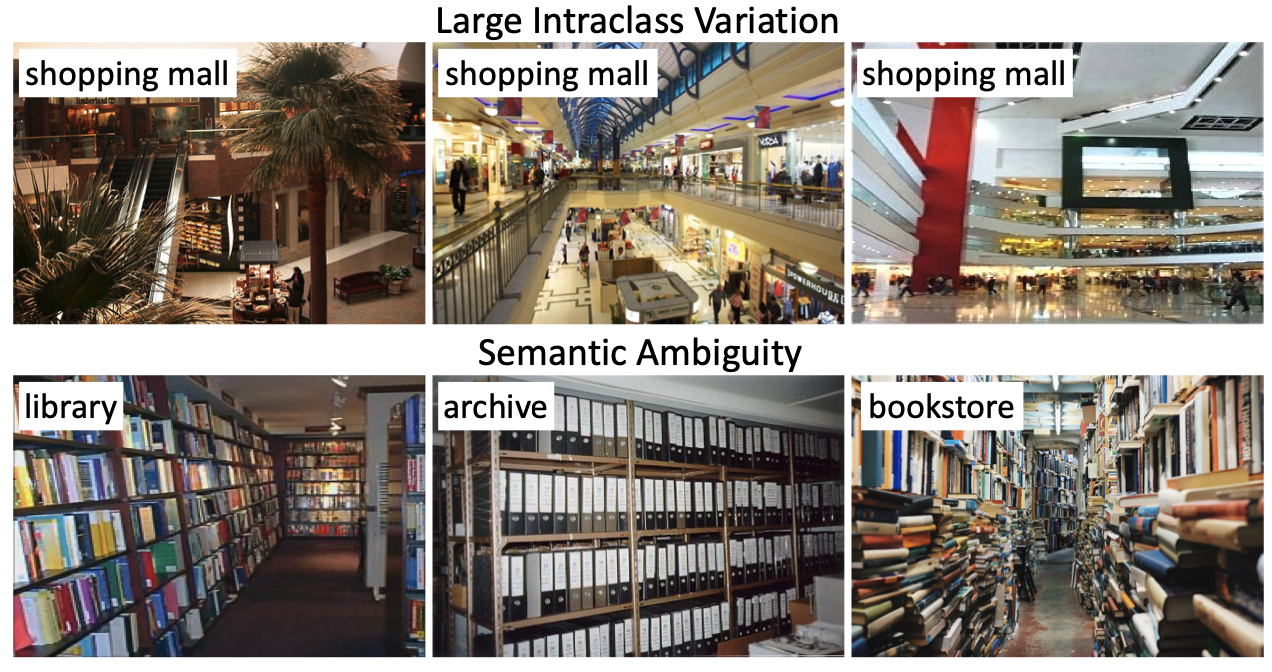
\includegraphics[width=\textwidth]{img/scene_class.png}
    \caption{Problem różnorodności wewnątrzklasowej oraz wieloznaczności semantycznej \cite{zeng2021deep}.}
    \label{fig:scene-class}
\end{figure}

Zadanie klasyfikacji sceny polega na przyporządkowaniu kategorii miejsca, w które przedstawia obraz. Istnieje duża różnica między klasyfikacja obrazka a klasyfikacją sceny. Klasyfikacja obrazka jako taka zajmuje się przyporządkowaniem klasy obiektu pierwszoplanowego, np. czy na obrazie znajduje się pies, czy kot. Klasyfikacja sceny natomiast musi wziąć pod uwagę wszystkie cechy obrazu, zarówno tła, jak i pierwszego planu, by określić odpowiednie miejsce. 

W kontekście środowisk wewnętrznych, klasyfikacja scen stanowi wyzwanie ze względu na zmienność scen wewnętrznych, obecność okluzji oraz fakt, że ten sam typ sceny może wyglądać inaczej na różnych obrazach. Wyróżniamy między innymi problem różnorodności wewnątrz klasowej oraz wieloznaczności semantycznej, co zostało przedstawione na rys. \ref{fig:scene-class}. Pierwszy z nich polega na fakcie, iż jedno miejsce może zostać przedstawione w bardzo różnej konfiguracji m.in. oświetlenia, ekspozycji, obiektów znajdujących się na obrazie. Drugi jest związany z występowaniem tych samych obiektów dla różnych klas scen.

\subsection{Segmentacja obrazu}
\begin{figure}[ht!]
    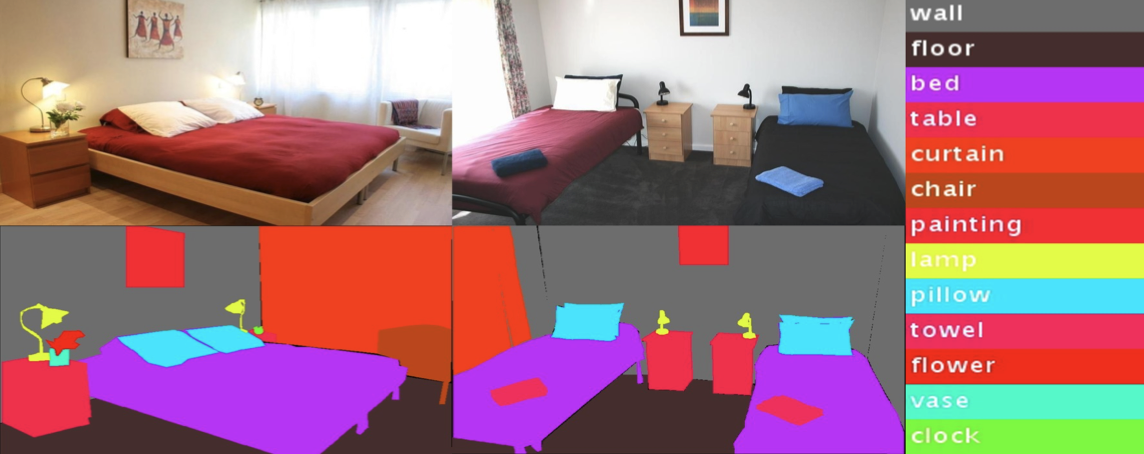
\includegraphics[width=\textwidth]{img/segment.png}
    \caption{Segmentacja wewnątrz pomieszczeń \cite{zhang2018context}.}
    \label{fig:segment}
  \end{figure}
  
Zadanie segmentacji obrazu to przyporządkowanie każdemu pikselowi etykiety takiej jak ,,łóżko'', ,,kanapa'' lub ,,umywalka'', do każdego piksela w obrazie (rys. \ref{fig:segment}). W rezultacie obraz zostaje podzielony na homogeniczne regiony pod względem pewnych własności. Segmentacja może być reprezentowana jako tablica 2D, gdzie każdy element odpowiada pikselowi w obrazie wejściowym i ma wartość wskazującą jego etykietę klasy.
  
Zadanie segmentacji można rozszerzyć do zadania segmentacji instancji (ang. instance segmentation), czyli segmentacji klasycznej rozszerzonej o rożróżnienie poszczególnych obiektów w ramach tej samej klasy. W przypadku klasycznej wersji nie jesteśmy w stanie rozróżnić dwóch stojących obok siebie łóżek, gdyż mapa segmentacji jest dla nich jednakowa. Segmentacja instacji pozwala natomiast takie rozróznienie uczynić. Segmentacja semtantyczna w dalszej części pracy będzie odnosić się do klasycznej wersji. Segmentacja instancji nie jest tematem pracy.

\subsection{Głębokie uczenie i konwolucje}
% # TODO 
\subsection{Uczenie wielozadaniowe}
% # TODO